% GNUPLOT: LaTeX picture with Postscript
\begingroup
  % Encoding inside the plot.  In the header of your document, this encoding
  % should to defined, e.g., by using
  % \usepackage[cp1252,<other encodings>]{inputenc}
  % \inputencoding{cp1252}%
  \makeatletter
  \providecommand\color[2][]{%
    \GenericError{(gnuplot) \space\space\space\@spaces}{%
      Package color not loaded in conjunction with
      terminal option `colourtext'%
    }{See the gnuplot documentation for explanation.%
    }{Either use 'blacktext' in gnuplot or load the package
      color.sty in LaTeX.}%
    \renewcommand\color[2][]{}%
  }%
  \providecommand\includegraphics[2][]{%
    \GenericError{(gnuplot) \space\space\space\@spaces}{%
      Package graphicx or graphics not loaded%
    }{See the gnuplot documentation for explanation.%
    }{The gnuplot epslatex terminal needs graphicx.sty or graphics.sty.}%
    \renewcommand\includegraphics[2][]{}%
  }%
  \providecommand\rotatebox[2]{#2}%
  \@ifundefined{ifGPcolor}{%
    \newif\ifGPcolor
    \GPcolorfalse
  }{}%
  \@ifundefined{ifGPblacktext}{%
    \newif\ifGPblacktext
    \GPblacktexttrue
  }{}%
  % define a \g@addto@macro without @ in the name:
  \let\gplgaddtomacro\g@addto@macro
  % define empty templates for all commands taking text:
  \gdef\gplbacktext{}%
  \gdef\gplfronttext{}%
  \makeatother
  \ifGPblacktext
    % no textcolor at all
    \def\colorrgb#1{}%
    \def\colorgray#1{}%
  \else
    % gray or color?
    \ifGPcolor
      \def\colorrgb#1{\color[rgb]{#1}}%
      \def\colorgray#1{\color[gray]{#1}}%
      \expandafter\def\csname LTw\endcsname{\color{white}}%
      \expandafter\def\csname LTb\endcsname{\color{black}}%
      \expandafter\def\csname LTa\endcsname{\color{black}}%
      \expandafter\def\csname LT0\endcsname{\color[rgb]{1,0,0}}%
      \expandafter\def\csname LT1\endcsname{\color[rgb]{0,1,0}}%
      \expandafter\def\csname LT2\endcsname{\color[rgb]{0,0,1}}%
      \expandafter\def\csname LT3\endcsname{\color[rgb]{1,0,1}}%
      \expandafter\def\csname LT4\endcsname{\color[rgb]{0,1,1}}%
      \expandafter\def\csname LT5\endcsname{\color[rgb]{1,1,0}}%
      \expandafter\def\csname LT6\endcsname{\color[rgb]{0,0,0}}%
      \expandafter\def\csname LT7\endcsname{\color[rgb]{1,0.3,0}}%
      \expandafter\def\csname LT8\endcsname{\color[rgb]{0.5,0.5,0.5}}%
    \else
      % gray
      \def\colorrgb#1{\color{black}}%
      \def\colorgray#1{\color[gray]{#1}}%
      \expandafter\def\csname LTw\endcsname{\color{white}}%
      \expandafter\def\csname LTb\endcsname{\color{black}}%
      \expandafter\def\csname LTa\endcsname{\color{black}}%
      \expandafter\def\csname LT0\endcsname{\color{black}}%
      \expandafter\def\csname LT1\endcsname{\color{black}}%
      \expandafter\def\csname LT2\endcsname{\color{black}}%
      \expandafter\def\csname LT3\endcsname{\color{black}}%
      \expandafter\def\csname LT4\endcsname{\color{black}}%
      \expandafter\def\csname LT5\endcsname{\color{black}}%
      \expandafter\def\csname LT6\endcsname{\color{black}}%
      \expandafter\def\csname LT7\endcsname{\color{black}}%
      \expandafter\def\csname LT8\endcsname{\color{black}}%
    \fi
  \fi
    \setlength{\unitlength}{0.0500bp}%
    \ifx\gptboxheight\undefined%
      \newlength{\gptboxheight}%
      \newlength{\gptboxwidth}%
      \newsavebox{\gptboxtext}%
    \fi%
    \setlength{\fboxrule}{0.5pt}%
    \setlength{\fboxsep}{1pt}%
\begin{picture}(4320.00,5760.00)%
    \gplgaddtomacro\gplbacktext{%
      \csname LTb\endcsname%%
      \put(300,3320){\makebox(0,0)[r]{\strut{}$0$}}%
      \put(300,3597){\makebox(0,0)[r]{\strut{}$1$}}%
      \put(300,3875){\makebox(0,0)[r]{\strut{}$2$}}%
      \put(300,4152){\makebox(0,0)[r]{\strut{}$3$}}%
      \put(300,4430){\makebox(0,0)[r]{\strut{}$4$}}%
      \put(300,4707){\makebox(0,0)[r]{\strut{}$5$}}%
      \put(300,4984){\makebox(0,0)[r]{\strut{}$6$}}%
      \put(300,5262){\makebox(0,0)[r]{\strut{}$7$}}%
      \put(300,5539){\makebox(0,0)[r]{\strut{}$8$}}%
      \put(432,3100){\makebox(0,0){\strut{}$-2$}}%
      \put(868,3100){\makebox(0,0){\strut{}$-1.5$}}%
      \put(1305,3100){\makebox(0,0){\strut{}$-1$}}%
      \put(1741,3100){\makebox(0,0){\strut{}$-0.5$}}%
      \put(2178,3100){\makebox(0,0){\strut{}$0$}}%
      \put(2614,3100){\makebox(0,0){\strut{}$0.5$}}%
      \put(3050,3100){\makebox(0,0){\strut{}$1$}}%
      \put(3487,3100){\makebox(0,0){\strut{}$1.5$}}%
      \put(3923,3100){\makebox(0,0){\strut{}$2$}}%
      \put(676,5428){\makebox(0,0)[l]{\strut{}(a)}}%
    }%
    \gplgaddtomacro\gplfronttext{%
      \csname LTb\endcsname%%
      \put(-52,4429){\rotatebox{-270}{\makebox(0,0){\strut{}$G/G_0$}}}%
      \csname LTb\endcsname%%
      \put(2936,5366){\makebox(0,0)[r]{\strut{}Pristine-$\beta_{12}$}}%
      \csname LTb\endcsname%%
      \put(2936,5146){\makebox(0,0)[r]{\strut{}V=1 eV}}%
      \csname LTb\endcsname%%
      \put(2936,4926){\makebox(0,0)[r]{\strut{}V=2 eV}}%
      \csname LTb\endcsname%%
      \put(2936,4706){\makebox(0,0)[r]{\strut{}V=5 eV}}%
    }%
    \gplgaddtomacro\gplbacktext{%
      \csname LTb\endcsname%%
      \put(300,704){\makebox(0,0)[r]{\strut{}$0$}}%
      \put(300,1095){\makebox(0,0)[r]{\strut{}$0.1$}}%
      \put(300,1486){\makebox(0,0)[r]{\strut{}$0.2$}}%
      \put(300,1878){\makebox(0,0)[r]{\strut{}$0.3$}}%
      \put(300,2269){\makebox(0,0)[r]{\strut{}$0.4$}}%
      \put(300,2660){\makebox(0,0)[r]{\strut{}$0.5$}}%
      \put(432,484){\makebox(0,0){\strut{}$-2$}}%
      \put(868,484){\makebox(0,0){\strut{}$-1.5$}}%
      \put(1305,484){\makebox(0,0){\strut{}$-1$}}%
      \put(1741,484){\makebox(0,0){\strut{}$-0.5$}}%
      \put(2178,484){\makebox(0,0){\strut{}$0$}}%
      \put(2614,484){\makebox(0,0){\strut{}$0.5$}}%
      \put(3050,484){\makebox(0,0){\strut{}$1$}}%
      \put(3487,484){\makebox(0,0){\strut{}$1.5$}}%
      \put(3923,484){\makebox(0,0){\strut{}$2$}}%
      \put(676,2562){\makebox(0,0)[l]{\strut{}(b)}}%
    }%
    \gplgaddtomacro\gplfronttext{%
      \csname LTb\endcsname%%
      \put(-316,1682){\rotatebox{-270}{\makebox(0,0){\strut{}LDOS}}}%
      \put(2177,154){\makebox(0,0){\strut{}Energy(eV)}}%
    }%
    \gplbacktext
    \put(0,0){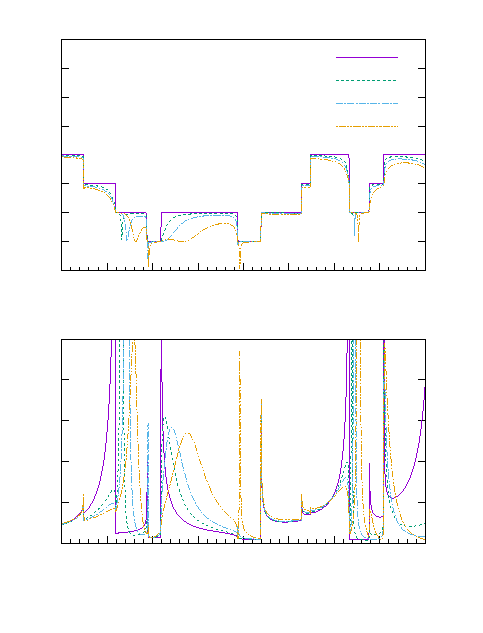
\includegraphics[width={217.00bp},height={289.00bp}]{armscatter}}%
    \gplfronttext
  \end{picture}%
\endgroup
